% Options for packages loaded elsewhere
\PassOptionsToPackage{unicode}{hyperref}
\PassOptionsToPackage{hyphens}{url}
\PassOptionsToPackage{dvipsnames,svgnames,x11names}{xcolor}
%
\documentclass[
  letterpaper,
  DIV=11,
  numbers=noendperiod]{scrartcl}

\usepackage{amsmath,amssymb}
\usepackage{iftex}
\ifPDFTeX
  \usepackage[T1]{fontenc}
  \usepackage[utf8]{inputenc}
  \usepackage{textcomp} % provide euro and other symbols
\else % if luatex or xetex
  \usepackage{unicode-math}
  \defaultfontfeatures{Scale=MatchLowercase}
  \defaultfontfeatures[\rmfamily]{Ligatures=TeX,Scale=1}
\fi
\usepackage{lmodern}
\ifPDFTeX\else  
    % xetex/luatex font selection
\fi
% Use upquote if available, for straight quotes in verbatim environments
\IfFileExists{upquote.sty}{\usepackage{upquote}}{}
\IfFileExists{microtype.sty}{% use microtype if available
  \usepackage[]{microtype}
  \UseMicrotypeSet[protrusion]{basicmath} % disable protrusion for tt fonts
}{}
\makeatletter
\@ifundefined{KOMAClassName}{% if non-KOMA class
  \IfFileExists{parskip.sty}{%
    \usepackage{parskip}
  }{% else
    \setlength{\parindent}{0pt}
    \setlength{\parskip}{6pt plus 2pt minus 1pt}}
}{% if KOMA class
  \KOMAoptions{parskip=half}}
\makeatother
\usepackage{xcolor}
\setlength{\emergencystretch}{3em} % prevent overfull lines
\setcounter{secnumdepth}{-\maxdimen} % remove section numbering
% Make \paragraph and \subparagraph free-standing
\makeatletter
\ifx\paragraph\undefined\else
  \let\oldparagraph\paragraph
  \renewcommand{\paragraph}{
    \@ifstar
      \xxxParagraphStar
      \xxxParagraphNoStar
  }
  \newcommand{\xxxParagraphStar}[1]{\oldparagraph*{#1}\mbox{}}
  \newcommand{\xxxParagraphNoStar}[1]{\oldparagraph{#1}\mbox{}}
\fi
\ifx\subparagraph\undefined\else
  \let\oldsubparagraph\subparagraph
  \renewcommand{\subparagraph}{
    \@ifstar
      \xxxSubParagraphStar
      \xxxSubParagraphNoStar
  }
  \newcommand{\xxxSubParagraphStar}[1]{\oldsubparagraph*{#1}\mbox{}}
  \newcommand{\xxxSubParagraphNoStar}[1]{\oldsubparagraph{#1}\mbox{}}
\fi
\makeatother


\providecommand{\tightlist}{%
  \setlength{\itemsep}{0pt}\setlength{\parskip}{0pt}}\usepackage{longtable,booktabs,array}
\usepackage{calc} % for calculating minipage widths
% Correct order of tables after \paragraph or \subparagraph
\usepackage{etoolbox}
\makeatletter
\patchcmd\longtable{\par}{\if@noskipsec\mbox{}\fi\par}{}{}
\makeatother
% Allow footnotes in longtable head/foot
\IfFileExists{footnotehyper.sty}{\usepackage{footnotehyper}}{\usepackage{footnote}}
\makesavenoteenv{longtable}
\usepackage{graphicx}
\makeatletter
\def\maxwidth{\ifdim\Gin@nat@width>\linewidth\linewidth\else\Gin@nat@width\fi}
\def\maxheight{\ifdim\Gin@nat@height>\textheight\textheight\else\Gin@nat@height\fi}
\makeatother
% Scale images if necessary, so that they will not overflow the page
% margins by default, and it is still possible to overwrite the defaults
% using explicit options in \includegraphics[width, height, ...]{}
\setkeys{Gin}{width=\maxwidth,height=\maxheight,keepaspectratio}
% Set default figure placement to htbp
\makeatletter
\def\fps@figure{htbp}
\makeatother

\usepackage{booktabs}
\usepackage{longtable}
\usepackage{array}
\usepackage{multirow}
\usepackage{wrapfig}
\usepackage{float}
\usepackage{colortbl}
\usepackage{pdflscape}
\usepackage{tabu}
\usepackage{threeparttable}
\usepackage{threeparttablex}
\usepackage[normalem]{ulem}
\usepackage{makecell}
\usepackage{xcolor}
\KOMAoption{captions}{tableheading}
\makeatletter
\@ifpackageloaded{caption}{}{\usepackage{caption}}
\AtBeginDocument{%
\ifdefined\contentsname
  \renewcommand*\contentsname{Table of contents}
\else
  \newcommand\contentsname{Table of contents}
\fi
\ifdefined\listfigurename
  \renewcommand*\listfigurename{List of Figures}
\else
  \newcommand\listfigurename{List of Figures}
\fi
\ifdefined\listtablename
  \renewcommand*\listtablename{List of Tables}
\else
  \newcommand\listtablename{List of Tables}
\fi
\ifdefined\figurename
  \renewcommand*\figurename{Figure}
\else
  \newcommand\figurename{Figure}
\fi
\ifdefined\tablename
  \renewcommand*\tablename{Table}
\else
  \newcommand\tablename{Table}
\fi
}
\@ifpackageloaded{float}{}{\usepackage{float}}
\floatstyle{ruled}
\@ifundefined{c@chapter}{\newfloat{codelisting}{h}{lop}}{\newfloat{codelisting}{h}{lop}[chapter]}
\floatname{codelisting}{Listing}
\newcommand*\listoflistings{\listof{codelisting}{List of Listings}}
\makeatother
\makeatletter
\makeatother
\makeatletter
\@ifpackageloaded{caption}{}{\usepackage{caption}}
\@ifpackageloaded{subcaption}{}{\usepackage{subcaption}}
\makeatother

\ifLuaTeX
  \usepackage{selnolig}  % disable illegal ligatures
\fi
\usepackage{bookmark}

\IfFileExists{xurl.sty}{\usepackage{xurl}}{} % add URL line breaks if available
\urlstyle{same} % disable monospaced font for URLs
\hypersetup{
  pdftitle={PM566 - Final},
  pdfauthor={Jazmin Hernandez},
  colorlinks=true,
  linkcolor={blue},
  filecolor={Maroon},
  citecolor={Blue},
  urlcolor={Blue},
  pdfcreator={LaTeX via pandoc}}


\title{PM566 - Final}
\author{Jazmin Hernandez}
\date{2024-12-06}

\begin{document}
\maketitle


\subsection{Introduction}\label{introduction}

The dataset Nutrition, Physical Activity, and Obesity, was acquired from
the Centers for Disease Control and Prevention through the Youth Risk
Behavior Surveillance System. In this dataset, there is information on
high school students in grades 9-12 from public and private schools
regarding their diet, physical activity, and weight. This data helps
inform the Division of Nutrition, Physical Activity, and Obesity which
in turn contributes to national and state data on these markers.

Background info on obesity and ethnicity and by state: Current research
shows that non-Hispanic Black adults have a higher prevalence of obesity
followed by Hispanic adults. Midwestern and Southern regions have a
higher prevalence of obesity according to the Centers for Disease
Control and Prevention. The goal of this analysis is to analyze if the
data collected from high school students through the Youth Risk Behavior
Surveillance System follows shows a trend for obesity and
state/ethnicity. For my analysis I will be exploring the following
questions:

\begin{enumerate}
\def\labelenumi{\arabic{enumi})}
\tightlist
\item
  Does obesity and weight status differ by state?
\item
  Does obesity and weight status differ by ethnicity?
\end{enumerate}

\subsection{Methods}\label{methods}

Can I also include summary stats of mean percent per question by
locationdesc

\subsubsection{How and Where the Data were
Acquired}\label{how-and-where-the-data-were-acquired}

The data were acquired from the Youth Risk Behavior Surveillance System
where surveys were given to national, state, territorial, tribal, and
large urban schools from grades 9-12 in U.S. high schools. Students were
randomly selected to participate based on their required classes or a
specific period of the school day. I used the API pertaining to the data
but had to modify the default limit to allow all 44,702 observations and
31 columns to allow for all data to be analyzed with no limit.

\subsubsection{Missing Values and Filtering
Data}\label{missing-values-and-filtering-data}

I assessed missing values for the key variables which
included:locationdesc, geolocation, data\_value, race\_ethnicity, class,
and question. I then filtered the dataset for only relevant class
observations including ``Obesity/Weight Status.'' Because this analysis
is focusing on obesity/weight pertaining to state and ethnicity, I kept
only relevant key variables mentioned above.

\subsubsection{Transformation from Longer to
Wider}\label{transformation-from-longer-to-wider}

To better visualize and compare data, I transformed the variable
``question'' into a binary variable where 1 = ``Percent of students in
grades 9-12 who have an overweight classification'' and 2 = ``Percent of
students in grades 9-12 who have obesity.'' To include more variables
rather than observations, I transformed the data from longer to wider.
By aggregating the data so that each column had a single data\_value, I
created Question 1 and Question 2 as two separate variables so that each
location pertaining to the obesity/weight status has a column for
Question 1 and another for Question 2 with their corresponding data
values in percentages.

\subsubsection{Exploratory Data Analysis
Tools}\label{exploratory-data-analysis-tools}

For exploratory data analysis, I used ggplots and bar plots to assess
individual variables and explore their distribution. From here I
discovered that the questions had equal counts, NY had the highest data
value counts, and the race/ethnicity that was most common in this sample
was Non-Hispanic White individuals.

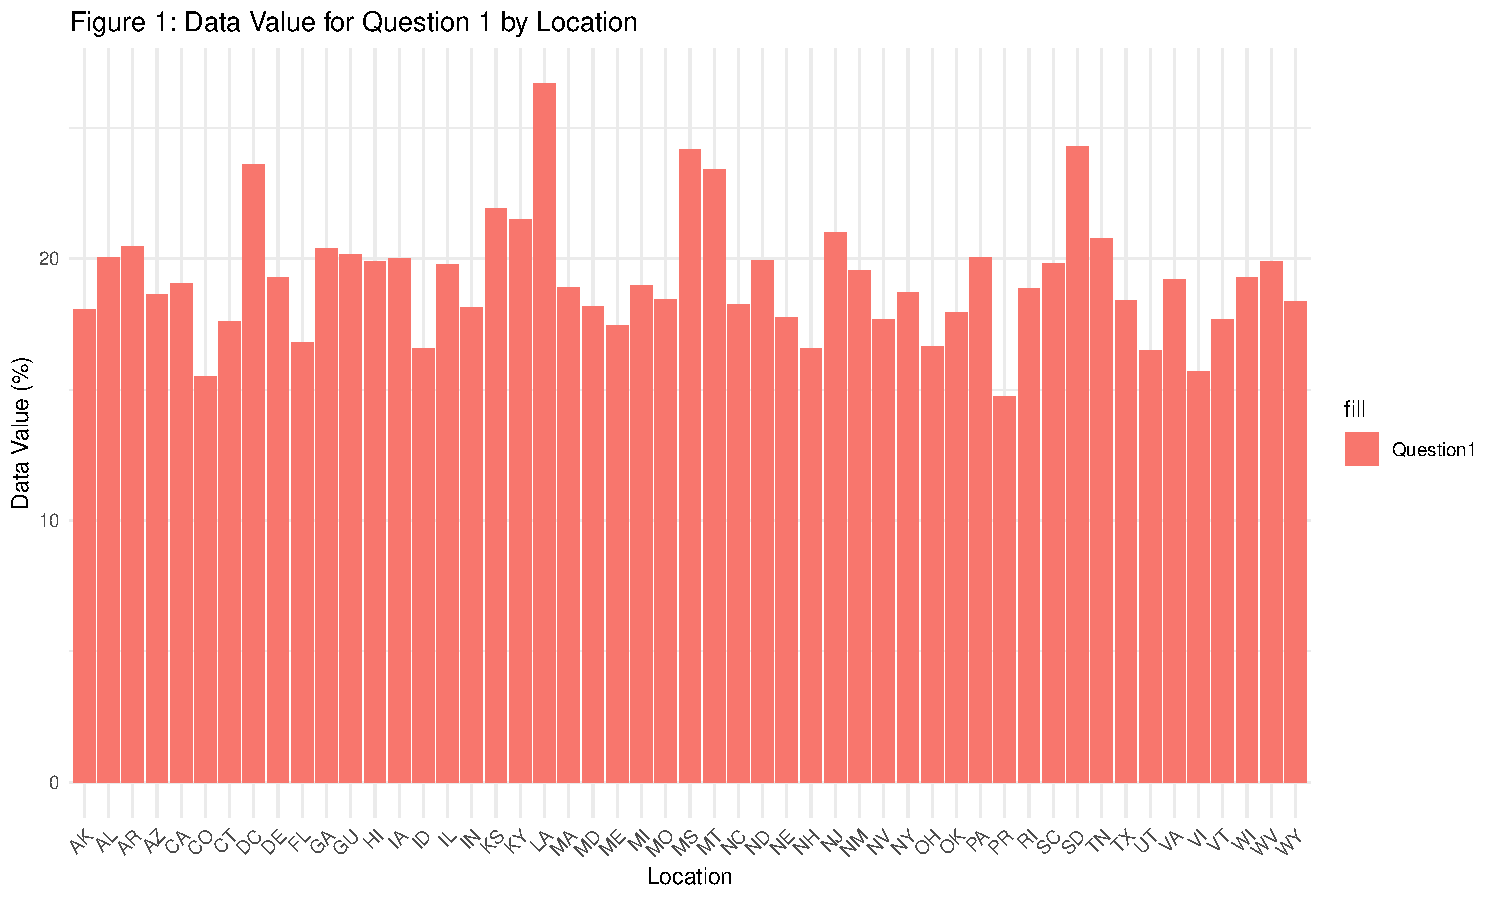
\includegraphics{PM566---Final_files/figure-pdf/unnamed-chunk-18-1.pdf}

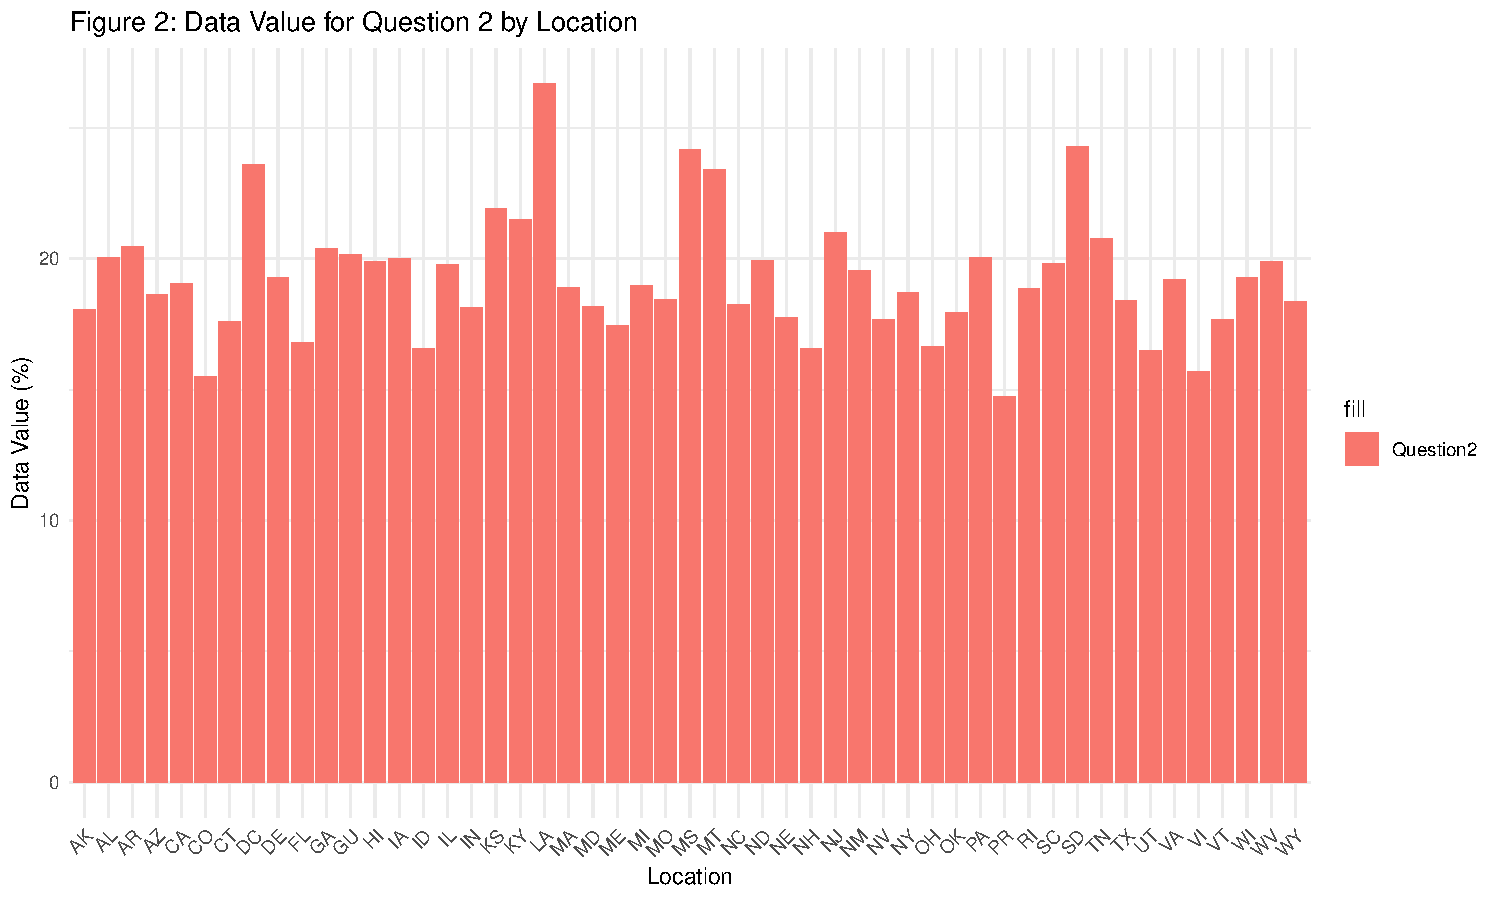
\includegraphics{PM566---Final_files/figure-pdf/unnamed-chunk-19-1.pdf}

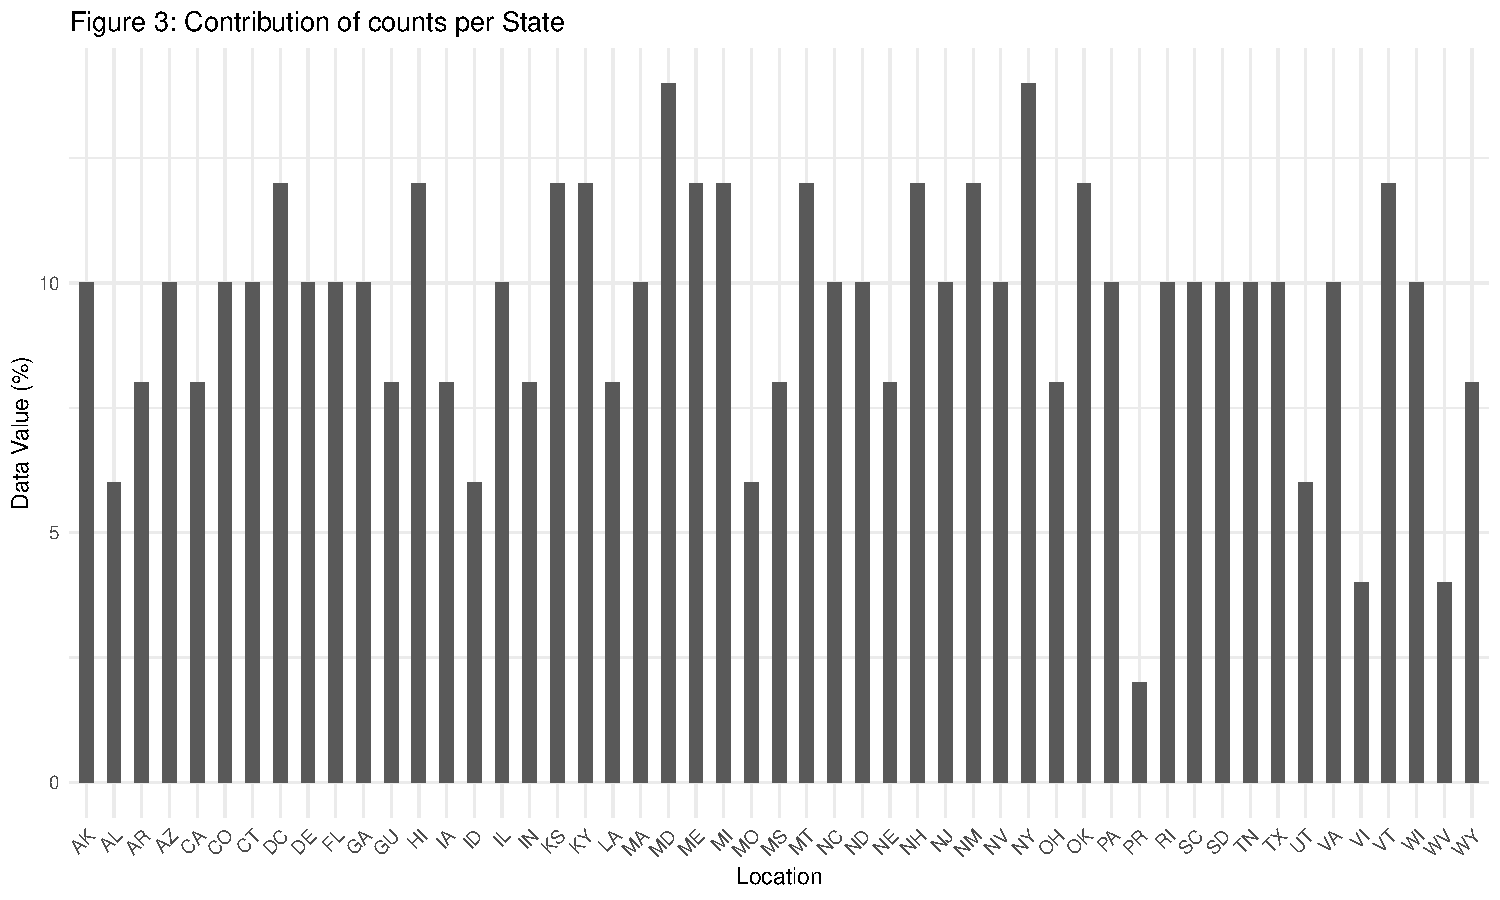
\includegraphics{PM566---Final_files/figure-pdf/unnamed-chunk-20-1.pdf}

\begin{verbatim}

Attaching package: 'kableExtra'
\end{verbatim}

\begin{verbatim}
The following object is masked from 'package:dplyr':

    group_rows
\end{verbatim}

\begin{longtable}[t]{lrrrrr}
\caption{Table 1: Summary Statistics for Location and Question}\\
\toprule
locationabbr & questions\_coded & Mean & Median & Count & SD\\
\midrule
MS & 2 & 21.890278 & 22.977778 & 4 & 5.0485714\\
GU & 2 & 20.491667 & 20.033333 & 4 & 3.4792906\\
LA & 1 & 20.241071 & 19.146429 & 4 & 4.7195583\\
ND & 2 & 18.651515 & 19.550000 & 5 & 4.8538149\\
MS & 1 & 18.631944 & 18.163889 & 4 & 4.1857351\\
\addlinespace
OH & 2 & 18.523214 & 17.525000 & 4 & 5.4775093\\
KS & 2 & 18.435417 & 17.943750 & 6 & 5.9968764\\
IN & 2 & 18.390952 & 18.520000 & 4 & 4.1110703\\
AL & 1 & 18.325926 & 19.377778 & 3 & 2.4119643\\
KS & 1 & 18.320417 & 18.461250 & 6 & 2.8378339\\
\addlinespace
IA & 2 & 18.239583 & 18.150000 & 4 & 4.4918000\\
KY & 1 & 18.160370 & 18.227778 & 6 & 2.1508725\\
AR & 1 & 18.050625 & 18.070000 & 4 & 2.1373858\\
WV & 1 & 17.905000 & 17.905000 & 2 & 2.8213561\\
KY & 2 & 17.875185 & 17.858333 & 6 & 5.3262702\\
\addlinespace
SD & 1 & 17.851333 & 17.450000 & 5 & 4.0540628\\
AR & 2 & 17.675625 & 17.720000 & 4 & 1.3639257\\
SC & 1 & 17.476444 & 19.460000 & 5 & 2.9052713\\
TN & 1 & 17.424333 & 17.775000 & 5 & 2.4455116\\
AL & 2 & 17.400000 & 18.388889 & 3 & 4.4444028\\
\addlinespace
PA & 1 & 17.136667 & 18.700000 & 5 & 2.9909623\\
TN & 2 & 16.912000 & 19.600000 & 5 & 5.9993100\\
MO & 1 & 16.867407 & 17.840000 & 3 & 2.2080731\\
WI & 1 & 16.836048 & 17.275000 & 5 & 2.1019907\\
IN & 1 & 16.640714 & 16.850000 & 4 & 1.6002863\\
\addlinespace
OK & 2 & 16.618102 & 17.707500 & 6 & 2.5065889\\
DC & 1 & 16.489583 & 16.762500 & 6 & 5.6855102\\
RI & 1 & 16.479299 & 17.640000 & 5 & 2.4339589\\
GA & 2 & 16.397857 & 17.000000 & 5 & 2.7490401\\
NJ & 1 & 16.397143 & 17.585714 & 5 & 3.8011867\\
\addlinespace
ND & 1 & 16.379242 & 17.550000 & 5 & 3.6709232\\
NE & 1 & 16.346875 & 16.900000 & 4 & 1.7375862\\
VI & 2 & 16.200000 & 16.200000 & 2 & 5.3740115\\
AK & 1 & 16.173333 & 16.600000 & 5 & 1.6523384\\
MO & 2 & 16.141482 & 17.360000 & 3 & 2.2721419\\
\addlinespace
CT & 1 & 16.034444 & 16.750000 & 5 & 1.8650638\\
GU & 1 & 16.016667 & 16.450000 & 4 & 3.7758001\\
IA & 1 & 15.950000 & 14.950000 & 4 & 2.7525746\\
OK & 1 & 15.922222 & 16.754167 & 6 & 2.1782377\\
VA & 1 & 15.843333 & 15.900000 & 5 & 3.2186652\\
\addlinespace
MT & 1 & 15.836239 & 15.865079 & 6 & 4.5720687\\
NC & 1 & 15.731636 & 16.472727 & 5 & 2.6006841\\
DE & 2 & 15.686000 & 16.600000 & 5 & 2.2247539\\
DE & 1 & 15.668000 & 18.190000 & 5 & 4.4222246\\
LA & 2 & 15.653571 & 15.350000 & 4 & 1.8726232\\
\addlinespace
GA & 1 & 15.539643 & 15.800000 & 5 & 4.3864316\\
VI & 1 & 15.500000 & 15.500000 & 2 & 0.2828427\\
MI & 1 & 15.431840 & 15.895454 & 6 & 3.4581680\\
AZ & 1 & 15.406000 & 17.310000 & 5 & 3.3326536\\
MA & 1 & 15.371515 & 16.866667 & 5 & 4.1946699\\
\addlinespace
IL & 1 & 15.364167 & 17.025000 & 5 & 4.0738448\\
NM & 1 & 15.326389 & 15.612500 & 6 & 2.6610507\\
MD & 1 & 15.280884 & 15.840000 & 7 & 2.7601883\\
NV & 1 & 15.222143 & 14.900000 & 5 & 1.9625226\\
SD & 2 & 15.175333 & 15.566667 & 5 & 4.2002828\\
\addlinespace
NY & 1 & 15.123560 & 15.370000 & 7 & 2.8388393\\
ID & 1 & 15.039394 & 16.200000 & 3 & 2.3240449\\
HI & 1 & 14.961111 & 14.683333 & 6 & 3.3031579\\
NE & 2 & 14.896875 & 14.375000 & 4 & 2.8493123\\
VT & 1 & 14.889731 & 15.482222 & 6 & 2.3890904\\
\addlinespace
ME & 1 & 14.849783 & 15.200000 & 6 & 2.2102440\\
AZ & 2 & 14.824000 & 14.850000 & 5 & 4.6619234\\
PR & 1 & 14.750000 & 14.750000 & 1 & NA\\
ME & 2 & 14.736797 & 15.742857 & 6 & 3.5560622\\
AK & 2 & 14.550833 & 15.016667 & 5 & 2.6717471\\
\addlinespace
PA & 2 & 14.536667 & 16.233333 & 5 & 4.6397797\\
PR & 2 & 14.500000 & 14.500000 & 1 & NA\\
NH & 1 & 14.459167 & 14.190000 & 6 & 1.5646898\\
TX & 2 & 14.358889 & 14.933333 & 5 & 4.6318869\\
MI & 2 & 14.265527 & 15.193333 & 6 & 4.3111553\\
\addlinespace
FL & 1 & 14.044762 & 14.357143 & 5 & 2.9759340\\
WY & 1 & 14.019107 & 13.173214 & 4 & 3.2177940\\
CT & 2 & 13.993333 & 16.566667 & 5 & 4.8305011\\
TX & 1 & 13.987222 & 12.877778 & 5 & 3.9230010\\
UT & 1 & 13.962500 & 15.100000 & 3 & 3.2468013\\
\addlinespace
NC & 2 & 13.955636 & 14.881818 & 5 & 3.6487105\\
SC & 2 & 13.950667 & 14.000000 & 5 & 5.0538552\\
NH & 2 & 13.793333 & 14.187500 & 6 & 4.1587398\\
WV & 2 & 13.785000 & 13.785000 & 2 & 5.0699556\\
OH & 1 & 13.726190 & 13.535714 & 4 & 2.2572383\\
\addlinespace
IL & 2 & 13.477500 & 14.450000 & 5 & 3.8486138\\
WI & 2 & 13.414452 & 13.733333 & 5 & 2.0896007\\
RI & 2 & 13.388390 & 14.190000 & 5 & 2.6692186\\
VA & 2 & 13.360667 & 14.600000 & 5 & 4.3456219\\
CA & 2 & 13.350000 & 13.350000 & 4 & 5.4003086\\
\addlinespace
CA & 1 & 13.333333 & 11.983333 & 4 & 3.9077321\\
HI & 2 & 13.204630 & 12.888889 & 6 & 5.2737978\\
UT & 2 & 13.180000 & 13.250000 & 3 & 6.5552803\\
MD & 2 & 13.155601 & 14.520000 & 7 & 3.8342686\\
NM & 2 & 13.115807 & 13.819643 & 6 & 5.9504977\\
\addlinespace
VT & 2 & 12.891169 & 14.175000 & 6 & 3.9703721\\
WY & 2 & 12.750000 & 11.150000 & 4 & 5.2016023\\
MA & 2 & 12.515353 & 13.322222 & 5 & 3.7321363\\
NY & 2 & 12.337483 & 12.666667 & 7 & 3.0028566\\
DC & 2 & 12.212500 & 13.850000 & 6 & 5.3169893\\
\addlinespace
NV & 2 & 12.133571 & 12.800000 & 5 & 3.8756415\\
MT & 2 & 11.765628 & 13.321429 & 6 & 6.7307176\\
CO & 1 & 11.633333 & 9.833333 & 5 & 3.3791024\\
FL & 2 & 11.610447 & 11.771429 & 5 & 2.1064214\\
ID & 2 & 10.527273 & 8.600000 & 3 & 4.6974320\\
\addlinespace
NJ & 2 & 10.409048 & 9.000000 & 5 & 4.9775244\\
CO & 2 & 8.413333 & 6.900000 & 5 & 4.9545910\\
\bottomrule
\end{longtable}

\begin{figure}[H]

{\centering 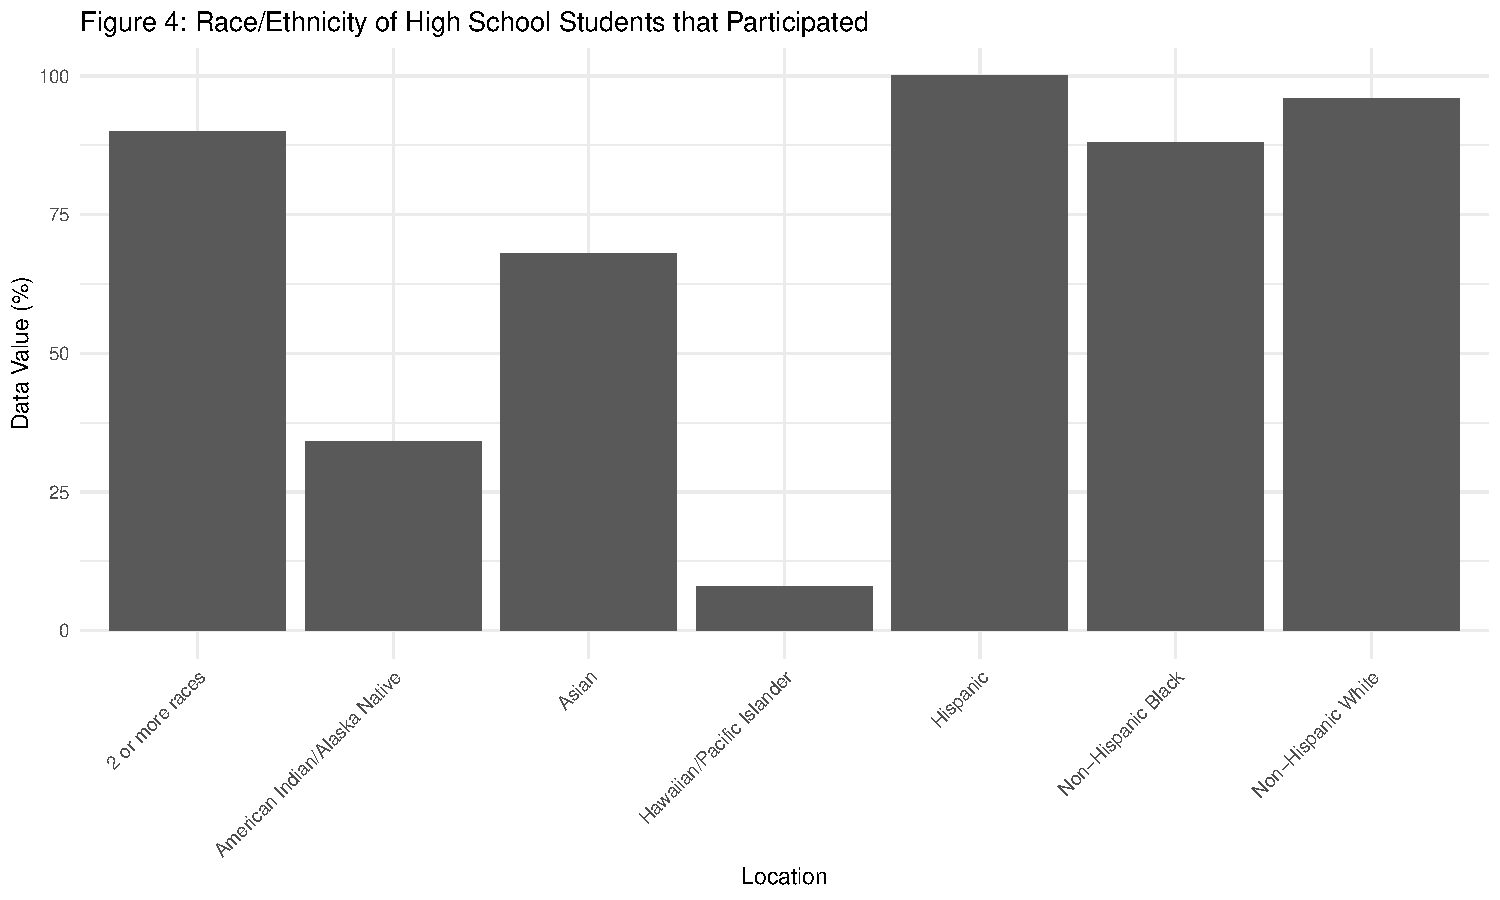
\includegraphics{PM566---Final_files/figure-pdf/unnamed-chunk-22-1.pdf}

}

\caption{This is a smaller bar plot.}

\end{figure}%

\begin{longtable}[t]{lrrrrr}
\caption{Table 2: Summary Statistics for Race/Ethnicity and Question}\\
\toprule
race\_ethnicity & questions\_coded & Mean & Median & Count & SD\\
\midrule
American Indian/Alaska Native & 2 & 18.955033 & 18.50000 & 17 & 4.412538\\
Hawaiian/Pacific Islander & 2 & 18.587540 & 19.04889 & 4 & 6.164833\\
Non-Hispanic Black & 1 & 17.701772 & 17.98939 & 44 & 2.020579\\
American Indian/Alaska Native & 1 & 17.699734 & 17.45000 & 17 & 2.517201\\
Hispanic & 1 & 17.637082 & 17.80750 & 50 & 2.154198\\
\addlinespace
Hispanic & 2 & 17.140585 & 16.78896 & 50 & 2.860944\\
Non-Hispanic Black & 2 & 16.732314 & 17.40500 & 44 & 2.595401\\
2 or more races & 1 & 16.267992 & 16.20000 & 45 & 3.044253\\
Hawaiian/Pacific Islander & 1 & 16.224286 & 16.28667 & 4 & 3.290938\\
2 or more races & 2 & 15.170445 & 14.88182 & 45 & 3.805146\\
\addlinespace
Non-Hispanic White & 1 & 13.453582 & 13.67500 & 48 & 1.595103\\
Asian & 1 & 13.009645 & 12.20000 & 34 & 3.783425\\
Non-Hispanic White & 2 & 11.234926 & 11.49886 & 48 & 2.805701\\
Asian & 2 & 9.188049 & 7.86250 & 34 & 4.466382\\
\bottomrule
\end{longtable}

\subsection{Results}\label{results}

\subsubsection{Figure 1}\label{figure-1}

To help with data visualization, I separated states into regions
pertaining to Northeast, Midwest, South, and West. From here, I was able
to create a bar plot with the average data values according to Question
1 and Question 2 stratified by region. This visual helped in determining
the first part of my question if obesity/weight status differed by
state. To help answer the second part of my question, I created another
bar plot of average data value by race/ethnicity and question. For the
creation of maps to help visualize the association, I first separated
and cleaned the geolocation variable into latitude and longitude
columns. I created a preliminary visual map distribution of where the
surveys were administered in the U.S. high schools. I created summary
statistics in tabular form of race/ethnicity by question 1 and question
2 where 2 or more races, Asian, Hispanic, Non-Hispanic Black, and
Non-Hispanic White had higher mean data values for Question 1. American
Indian/Alaska Native and Hawaiian/Pacific Islander had higher mean data
values for question 2.

To create a final representation to help answer my question, I filtered
the data to include Question 1 and Question 2 separately. I then created
separate maps to visualize the distribution of ethnicity/race and mean
data values of the questions separately. By doing this, I could interact
with the map and compare the mean data values (in percent) of how
obesity/weight status differed by location and by race/ethnicity. The
average data value percentage of obesity/weight for Question 1 was of
17.62\% in the following locations: Alaska, South Carolina, North
Carolina, Georgia, Michigan, and Wyoming. The race/ethnicity in all
these locations was American Indian/Alaska Native. For Question 2, the
percentage of obesity/weight status was again 17.62\% which was the
highest in North Dakota and Alaska. The ethnicity were also American
Indian/Alaska Native.

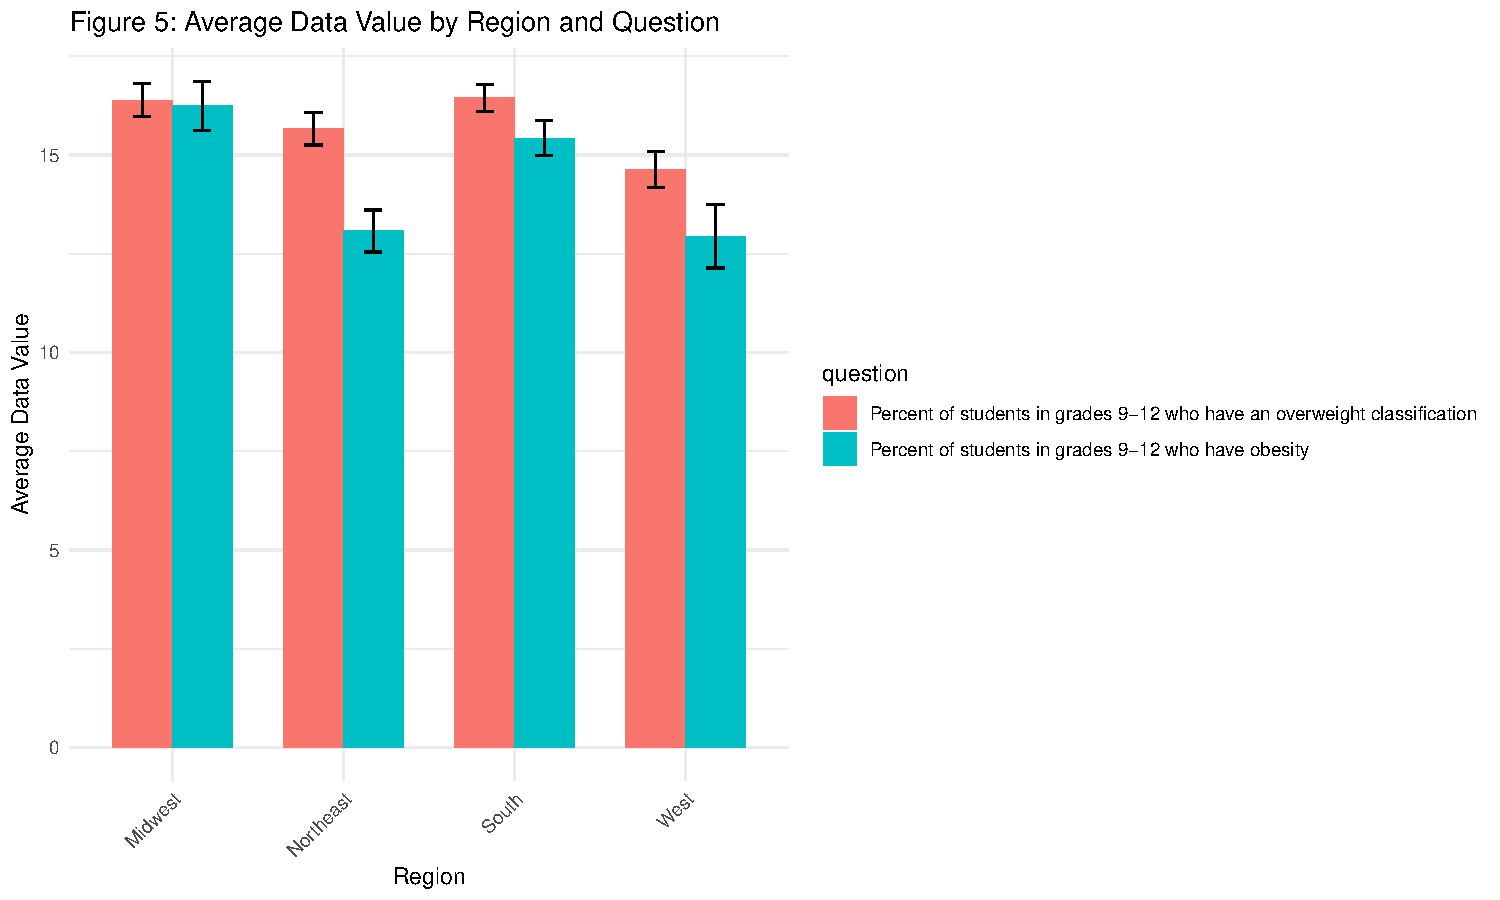
\includegraphics{PM566---Final_files/figure-pdf/unnamed-chunk-27-1.pdf}

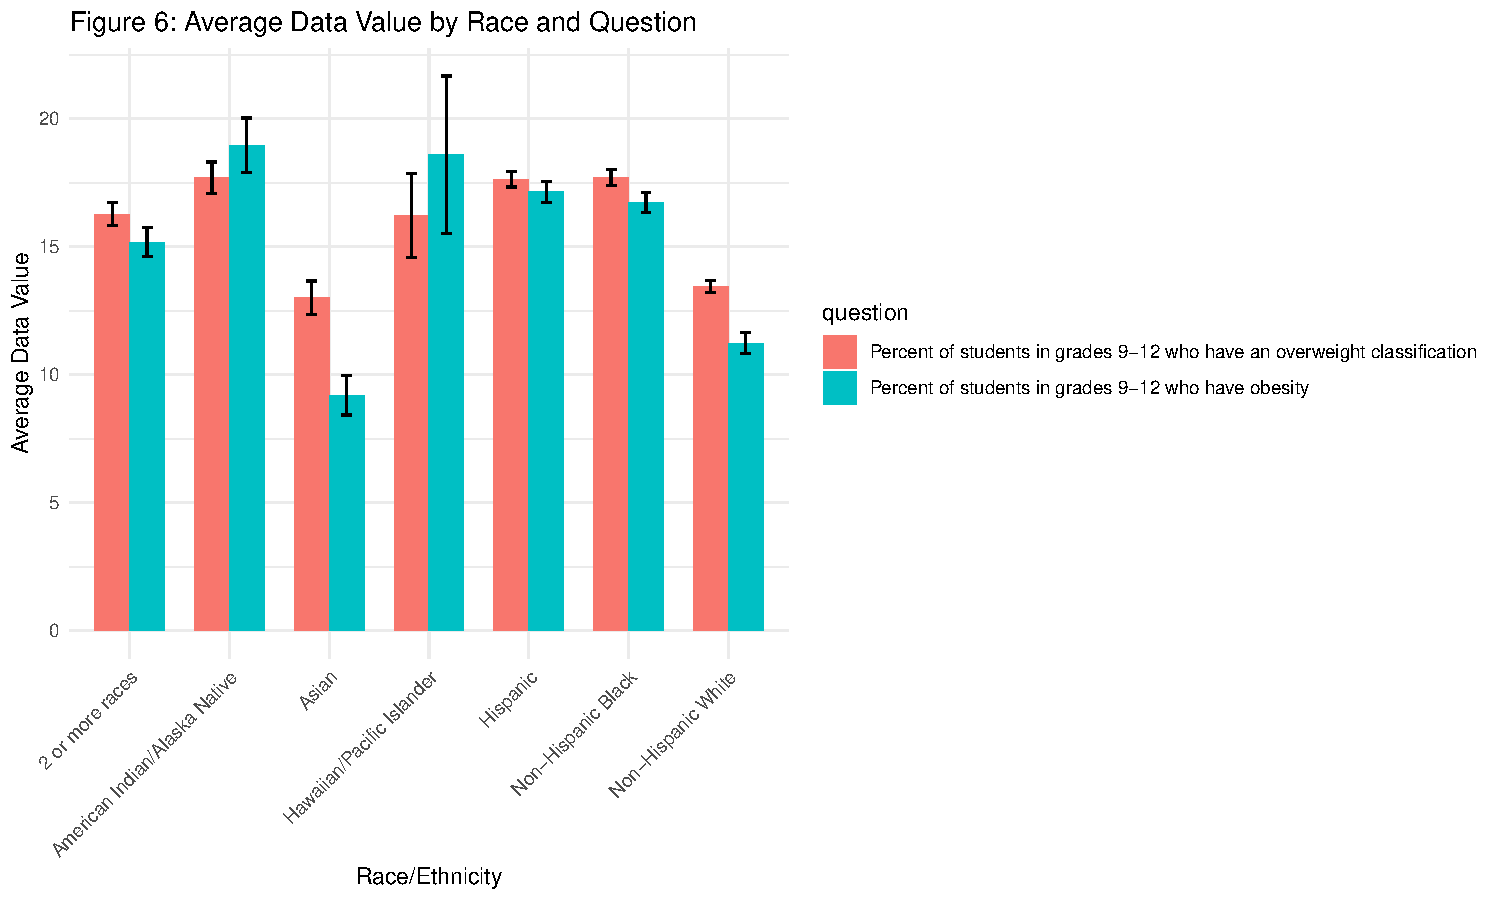
\includegraphics{PM566---Final_files/figure-pdf/unnamed-chunk-28-1.pdf}

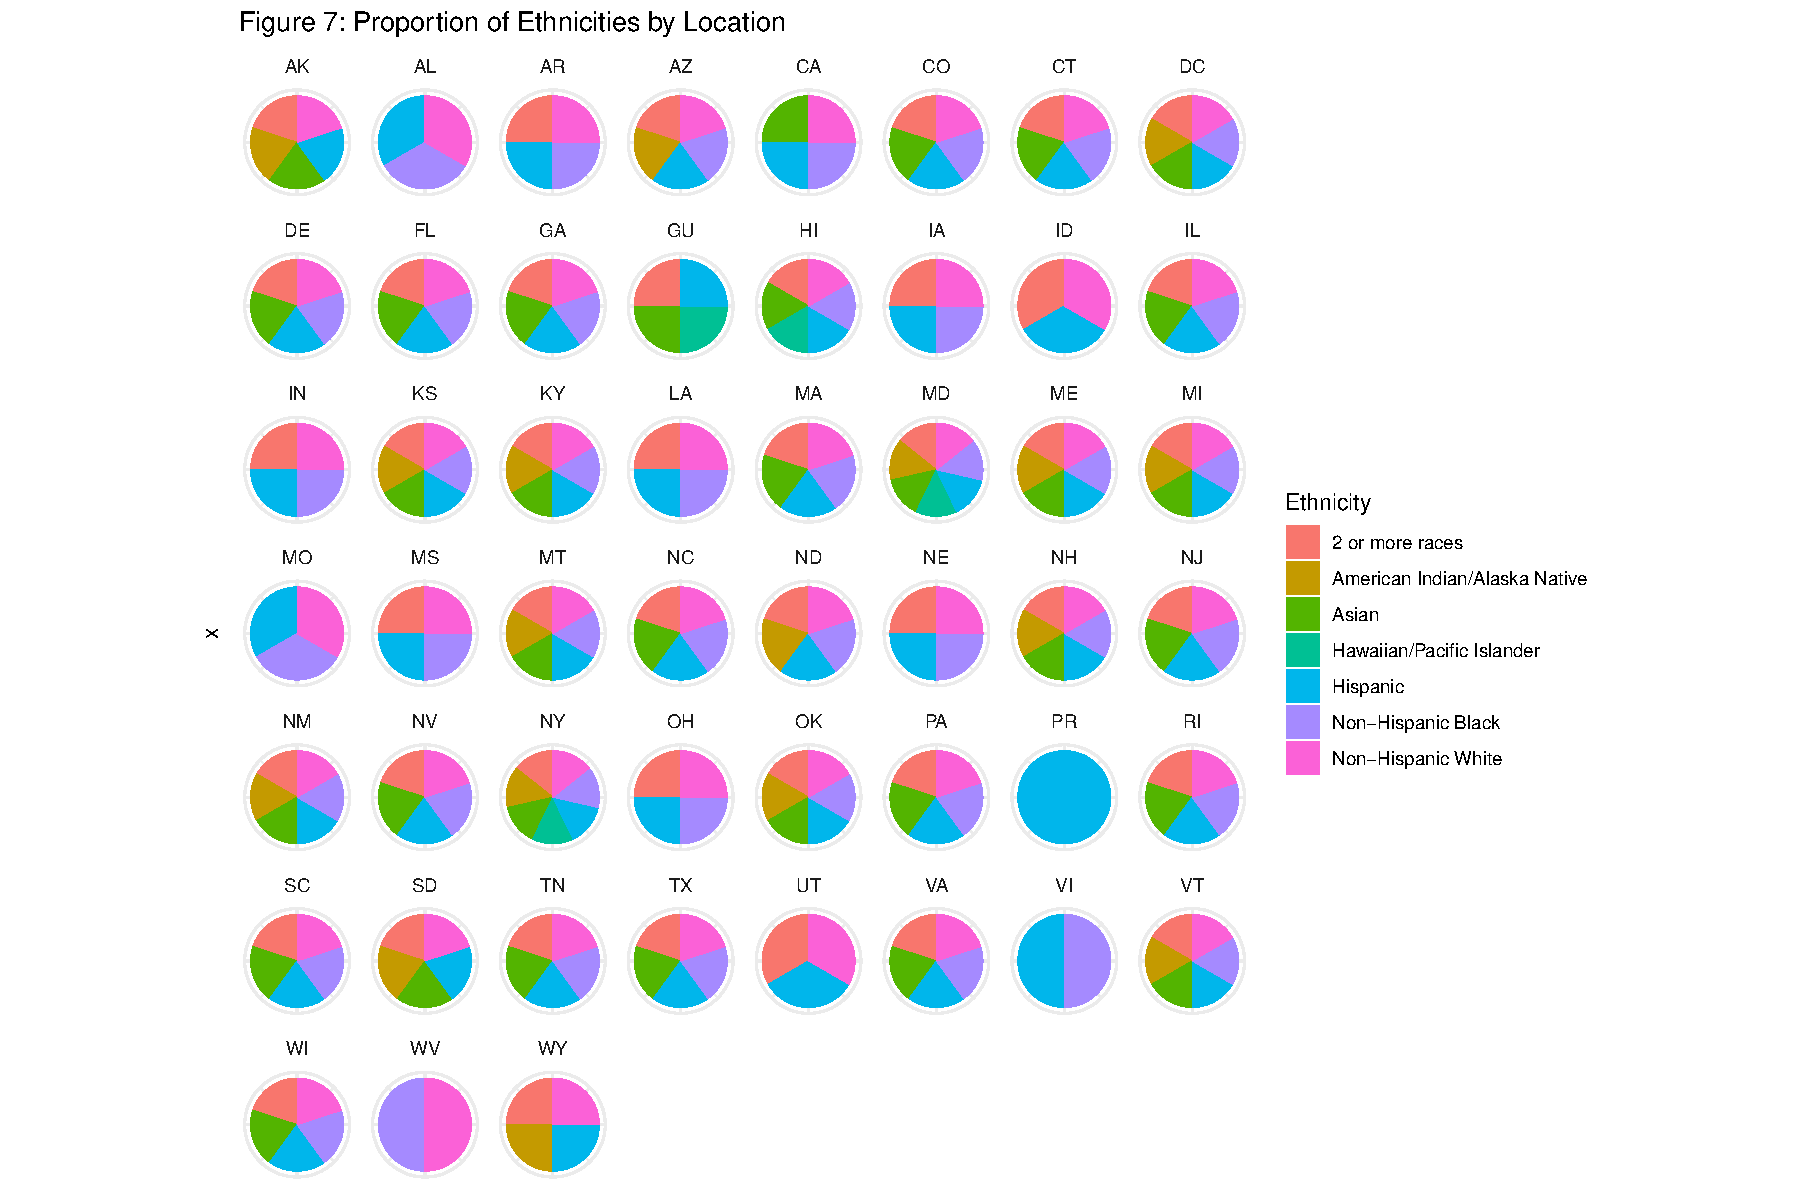
\includegraphics{PM566---Final_files/figure-pdf/unnamed-chunk-31-1.pdf}

\subsection{Conclusion}\label{conclusion}

After exploratory data analysis and the creation of graphs it appears
that obesity/weight status is higher in the American Indian/Alaska
Native population. This is true for Question 1 ``Percent of students in
grades 9-12 who have an overweight classification'' and Question 2
``Percent of students in grades 9-12 who have obesity.'' However, there
is a greater distribution of students falling into Question 1 category
as seen in that more states had a higher percent mean value of this
distribution compare to Question 2. This is also seen in the bar plot
comparing average data values by region stratified by question 1 and 2.
Question 1 appears to have a higher average data value than question 2
in all regions.

In summary, this data showed that\ldots. which is in line with the data
on obesity in adults according to ethnicity and place. From data such as
YRBSS published by CDC, programs can be implemented to help diminish the
obesity epidemic in adolescents. However, the data might not be
representative of the entire U.S. high school student population.
Although private, public, charter schools were included, some states had
minimal participation as seen in Fig\ldots.

\newpage

\subsection{References}\label{references}




\end{document}
